\documentclass[14pt]{extarticle}
\usepackage{fontspec}
\usepackage{polyglossia}
\usepackage{amsmath}
\usepackage{amssymb}
\usepackage{xcolor}
\usepackage{fancyhdr}
\usepackage{graphicx}
\usepackage{listings}
\usepackage[most]{tcolorbox}
% \usepackage{setspace}
\usepackage{pifont}
\usepackage{enumitem}
\usepackage{titlesec}
\usepackage[bottom]{footmisc}
\usepackage{titling}
\usepackage{minted}
\usepackage{etoolbox}
\usepackage{array}
\usepackage{longtable} % page-breakable tables (must load before polyglossia/bidi RTL setup)
\usepackage{extsizes}
\usepackage{float}
\usepackage{booktabs}
\usepackage{hyperref}
\usepackage[onehalfspacing]{setspace}
\newif\ifwhiteblack
\ifdefined\setwhiteblack
  \setwhiteblack
\fi

\ifwhiteblack
  \usepackage[a4paper, landscape, top=1.25cm, bottom=1.25cm, left=1.25cm, right=1.25cm, headheight=1.5cm, headsep=0.5cm]{geometry}
\else
  \usepackage[a4paper, top=2.7cm, bottom=2.7cm, left=2.5cm, right=2.5cm, headheight=1.5cm, headsep=0.5cm]{geometry}
\fi
\usepackage{tikz}
\usepackage{datetime2}

\usetikzlibrary{automata, positioning, arrows.meta, arrows}
\providecommand{\LTcaptype}{table}

\newfontfamily\emoji{Segoe UI Emoji}

\pagestyle{fancy}

\setmainlanguage[numerals=western]{arabic}
\setotherlanguage{english}
\newfontfamily\arabicfont[Script=Arabic]{Calibri}
\newfontfamily\arabicfonttt[Script=Arabic]{Courier New}



\ifwhiteblack
\lstset{
  language=[Sharp]C,
  numbers=left,
  stepnumber=1,
  numbersep=8pt,
  frame=single,
  basicstyle=\ttfamily\small,
  keywordstyle=\bfseries,
  stringstyle=\ttfamily,
  commentstyle=\itshape
}
\else
\lstset{
  language=[Sharp]C,
  numbers=left,
  stepnumber=1,
  numbersep=8pt,
  frame=single,
  basicstyle=\ttfamily\small,
  keywordstyle=\color{blue},
  stringstyle=\color{red},
  commentstyle=\color{green!50!black}
}
\fi

\newif\ifdetailed
\ifdefined\setdetailed
  \setdetailed
\fi

\newif\ifwithsols
\ifdefined\setwithsols
  \setwithsols
\fi

\ifwhiteblack
  \AtBeginDocument{
    \LARGE
    \usemintedstyle{bw}
  }
\fi

% Default minted look: compact code that wraps long lines.
% Not applied in black-and-white landscape mode, which already uses \LARGE.
\ifwhiteblack\else
  \setminted{fontsize=\small, breaklines=true}
\fi

% unified tcolorboxes for articles
\ifwhiteblack
\tcbset{colback=white, colframe=black, fonttitle=\bfseries, boxrule=1pt}
\newtcolorbox{boxDef}[1][]{title={{\emoji📘} تعريف\ifx\\#1\\\else ~#1\fi :}}
\newtcolorbox{boxExercise}[1][]{title={{\emoji🧩} تمرين\ifx\\#1\\\else ~#1\fi :}}
\newtcolorbox{boxExample}[1][]{title={{\emoji📝} مثال\ifx\\#1\\\else ~#1\fi :}}
\newtcolorbox{boxNote}[1][]{title={{\emoji✨} ملاحظة\ifx\\#1\\\else ~#1\fi :}}
\newtcolorbox{boxAttention}[1][]{title={{\emoji🔔} تنبيه\ifx\\#1\\\else ~#1\fi :}}
\newtcolorbox{boxWarning}[1][]{title={{\emoji⚡} ملاحظة هامة\ifx\\#1\\\else ~#1\fi :}}
\newtcolorbox{boxSolution}[1][]{title={{\emoji✅} حل\ifx\\#1\\\else ~#1\fi :}}
\newtcolorbox{boxSymbol}[1][]{title={{\emoji🔣} رمز\ifx\\#1\\\else ~#1\fi :}}
\newtcolorbox{boxHint}[1][]{title={{\emoji💡} تلميح\ifx\\#1\\\else ~#1\fi :}}
\else
\tcbset{colback=white, colframe=black, fonttitle=\bfseries, boxrule=0.8pt}
\newtcolorbox{boxDef}[1][]{colback=blue!5!white,colframe=blue!75!black,
  title={{\emoji📘} تعريف\ifx\\#1\\\else ~#1\fi :}}
\newtcolorbox{boxExercise}[1][]{colback=cyan!5!white,colframe=cyan!70!black,
  title={{\emoji🧩} تمرين\ifx\\#1\\\else ~#1\fi :}}
\newtcolorbox{boxExample}[1][]{colback=yellow!5!white,colframe=orange!90!black,
  title={{\emoji📝} مثال\ifx\\#1\\\else ~#1\fi :}}
\newtcolorbox{boxNote}[1][]{colback=gray!10!white,colframe=black,
  title={{\emoji✨} ملاحظة\ifx\\#1\\\else ~#1\fi :}}
\newtcolorbox{boxAttention}[1][]{colback=magenta!10!white,colframe=magenta!80!black,
  title={{\emoji🔔} تنبيه\ifx\\#1\\\else ~#1\fi :}}
\newtcolorbox{boxWarning}[1][]{colback=red!5!white,colframe=red!75!black,
  title={{\emoji⚡} ملاحظة هامة\ifx\\#1\\\else ~#1\fi :}}
\newtcolorbox{boxSolution}[1][]{colback=green!5!white,colframe=green!60!black,
  title={{\emoji✅} حل\ifx\\#1\\\else ~#1\fi :}}
\newtcolorbox{boxSymbol}[1][]{colback=purple!5!white,colframe=purple!70!black,
  title={{\emoji🔣} رمز\ifx\\#1\\\else ~#1\fi :}}
\newtcolorbox{boxHint}[1][]{colback=teal!5!white,colframe=teal!60!black,
  title={{\emoji💡} تلميح\ifx\\#1\\\else ~#1\fi :}}
\fi


\ifwhiteblack
\tcbset{simplecode/.style={ colback=white, colframe=black, boxrule=1pt, arc=2pt, left=4pt,right=4pt,top=4pt,bottom=4pt}}
\else
\tcbset{simplecode/.style={ colback=gray!5, colframe=black!50, boxrule=0.4pt, arc=2pt, left=4pt,right=4pt,top=4pt,bottom=4pt}}
\fi
% Compact code boxes: tighter line spacing (the preamble uses onehalfspacing) and small vertical gaps.
% Must come AFTER the simplecode definition above.
\tcbset{simplecode/.append style={fontupper=\setstretch{0.95}, top=4pt, bottom=4pt, before skip=6pt, after skip=6pt}}
\newenvironment{boxCode}{\begin{tcolorbox}[simplecode]}{\end{tcolorbox}}

% Code cell used inside tables (keeps code left-to-right inside RTL tables).
% Use inside a fixed-width p{...} column: \begin{pycell}\begin{minted}...\end{minted}\end{pycell}
\newtcolorbox{pycell}{frame empty,colback=white,boxsep=0pt,left=2pt,right=2pt,top=2pt,bottom=2pt,width=\linewidth}

\newcolumntype{C}[1]{>{\centering\arraybackslash}p{#1}}

\makeatletter
\DTMnewdatestyle{dotted}{%
  \renewcommand{\DTMdisplaydate}[4]{\two@digits{##3}.\two@digits{##2}.##1}%
  \renewcommand{\DTMDisplaydate}{\DTMdisplaydate}%
}
\makeatother
\DTMsetdatestyle{dotted}

% redefine spaces after titles
\makeatletter
\renewcommand{\@maketitle}{%
  \begin{center}
    {\huge \bfseries \@title \par}%
    \vskip 0.2em % space between title and author
    {\large \@author \par}%
    % \vskip 0.2em % space between author and date
    % {\normalsize \@date \par}%
    {\small \hfill \begin{english}\DTMtoday\end{english} \par}%
  \end{center}
}
\makeatother

\fancyhf{} % clear default
\fancypagestyle{plain}{
  \fancyhf{}
  \fancyhead[L]{مدرسة التسامح الشاملة}
  % \fancyhead[L]{
\includegraphics[height=1cm]{../../../images/logoTasamoh.png}}
  \fancyhead[R]{الأستاذ محمود اغبارية}
  \fancyfoot[C]{\thepage}
}

\fancyhead[L]{مدرسة التسامح الشاملة}
\fancyhead[R]{الأستاذ محمود اغبارية}
\fancyfoot[C]{\thepage}

\setcounter{tocdepth}{3} % only section subsection and subsubsection in TOC

\newcommand{\importpdfpage}[2]{%
    \thispagestyle{empty}
    \newgeometry{left=0cm,right=0cm,top=0cm,bottom=0cm}
    \includegraphics[page=#2,width=0.95\paperwidth,height=0.95\paperheight,keepaspectratio]{#1}
    \restoregeometry
}

\newcommand{\insertFullImg}[1]{%
    \noindent
    \makebox[\textwidth][c]{
        \includegraphics[width=0.9\paperwidth,keepaspectratio]{#1}%
    }%
}%


\ifwithsols
\title{حل ورقة تمرن $8$ للصف العاشر $10$ - العمليات الخارجية}
\else
\title{ورقة تمرن $8$ للصف العاشر $10$ - العمليات الخارجية}
\fi

\begin{document}

\maketitle
\thispagestyle{fancy}

\begin{boxAttention}
\begin{itemize}
    \item عندما يُطلب منك كتابة «عملية خارجية \textbf{تستقبل}»، يجب أن يكون المستخدم هو من يُدخل القيمة عبر لوحة المفاتيح، أي عليك استعمال \textenglish{Console.ReadLine()}.
    \item عندما يُطلب منك كتابة «عملية خارجية \textbf{تتلقى}»، فهذا يعني أنّ العملية تأخذ القيم كمعطيات (بارامترات) داخل القوسين في تعريف العملية.
    \item عندما يُطلب منك كتابة «برنامج»، فهذا يعني الكتابة داخل العملية الرئيسية \textenglish{Main()}.
    \item إذا كانت العملية \textbf{تعيد} قيمة ما (نمط الإرجاع ليس \textenglish{void})، فعليك حفظ القيمة المعادة في متغير عند استدعائها، أو طباعتها، أو استخدامها داخل تعبير أو شرط. أمّا إذا كانت العملية \textbf{لا تعيد} قيمة (\textenglish{void})، فإنّك تكتب اسمها فقط عند استدعائها وتمرّر لها المعطيات إن وُجدت.
\end{itemize}
\end{boxAttention}

% ==============================================================
% القسم الأول: عمليات لا تتلقى ولا تعيد - فقط تستقبل وتطبع
% ==============================================================
\section*{القسم الأوّل: عمليات لا تتلقى ولا تعيد}

\begin{enumerate}[itemsep=1em]

\item اكتب عملية خارجية لا تتلقى معطيات ولا تعيد قيمة، \textbf{تستقبل} اسم المستخدم \textbf{وتطبع} اسمه. ثم استدعِها في \textenglish{Main}.
\ifwithsols
\begin{boxSolution}
\begin{english}
\begin{minted}{csharp}
public static void ReadAndPrintName()
{
    Console.WriteLine("Enter your name:");
    string name = Console.ReadLine();
    Console.WriteLine(name);
}

public static void Main()
{
    ReadAndPrintName();
}
\end{minted}
\end{english}
\end{boxSolution}
\fi
\filbreak

\item اكتب عملية خارجية لا تتلقى معطيات ولا تعيد قيمة، \textbf{تستقبل} عددين صحيحين من المستخدم \textbf{وتطبع} مجموعهما. ثم استدعِها في \textenglish{Main}.
\ifwithsols
\begin{boxSolution}
\begin{english}
\begin{minted}{csharp}
public static void ReadAndPrintSum()
{
    Console.WriteLine("Enter two integers:");
    int a = int.Parse(Console.ReadLine());
    int b = int.Parse(Console.ReadLine());
    int sum = a + b;
    Console.WriteLine(sum);
}

public static void Main()
{
    ReadAndPrintSum();
}
\end{minted}
\end{english}
\end{boxSolution}
\fi
\filbreak

\item اكتب عملية خارجية لا تتلقى معطيات ولا تعيد قيمة، \textbf{تستقبل} من المستخدم عددًا صحيحًا موجبًا $n$، \textbf{وتطبع} الأعداد من $1$ إلى $n$ باستخدام حلقة \textenglish{for}. ثم استدعِها في \textenglish{Main}.
\ifwithsols
\begin{boxSolution}
\begin{english}
\begin{minted}{csharp}
public static void ReadAndPrintUpToN()
{
    Console.WriteLine("Enter n:");
    int n = int.Parse(Console.ReadLine());
    for (int i = 1; i <= n; i++)
    {
        Console.WriteLine(i);
    }
}

public static void Main()
{
    ReadAndPrintUpToN();
}
\end{minted}
\end{english}
\end{boxSolution}
\fi
\filbreak

\end{enumerate}

\clearpage
% ==============================================================
% القسم الثاني: عمليات تتلقى ولا تعيد (قسم منها يستقبل أيضًا)
% ==============================================================
\section*{القسم الثاني: عمليات تتلقى ولا تعيد}

\begin{enumerate}[resume, itemsep=1em]

\item اكتب عملية خارجية \textbf{تتلقى} عددًا صحيحًا \textbf{وتطبع} تربيعه (لا تعيد قيمة). ثم اكتب برنامجًا يستقبل عددًا صحيحًا من المستخدم ويستدعي العملية.
\ifwithsols
\begin{boxSolution}
\begin{english}
\begin{minted}{csharp}
public static void PrintSquare(int n)
{
    int sq = n * n;
    Console.WriteLine(sq);
}

public static void Main()
{
    int n = int.Parse(Console.ReadLine());
    PrintSquare(n);
}
\end{minted}
\end{english}
\end{boxSolution}
\fi
\filbreak

\item اكتب عملية خارجية \textbf{تتلقى} عددين عشريّين \textbf{وتطبع} معدّلهما (لا تعيد قيمة). ثم اكتب برنامجًا يستقبل عددين عشريّين من المستخدم ويستدعي العملية.
\ifwithsols
\begin{boxSolution}
\begin{english}
\begin{minted}{csharp}
public static void PrintAverageTwo(double a, double b)
{
    double avg = (a + b) / 2.0;
    Console.WriteLine(avg);
}

public static void Main()
{
    double a = double.Parse(Console.ReadLine());
    double b = double.Parse(Console.ReadLine());
    PrintAverageTwo(a, b);
}
\end{minted}
\end{english}
\end{boxSolution}
\fi
\filbreak

\item اكتب عملية خارجية \textbf{تتلقى} سعر منتج (\textenglish{double})، \textbf{وتستقبل} من المستخدم عدد القطع التي يريد شراءها (\textenglish{int})، ثم \textbf{تطبع} المبلغ الإجمالي للدفع (لا تعيد قيمة). ثم استدعِها في \textenglish{Main}.
\ifwithsols
\begin{boxSolution}
\begin{english}
\begin{minted}{csharp}
public static void PrintTotalCost(double price)
{
    Console.WriteLine("Enter quantity:");
    int quantity = int.Parse(Console.ReadLine());
    double total = price * quantity;
    Console.WriteLine("Total cost: " + total);
}

public static void Main()
{
    PrintTotalCost(15.5);
}
\end{minted}
\end{english}
\end{boxSolution}
\fi
\filbreak

\item اكتب عملية خارجية \textbf{تتلقى} عددًا صحيحًا موجبًا $n$، \textbf{وتطبع} الأعداد من $1$ حتى $n$، ولكن بدلاً من كل عدد يقبل القسمة على $4$ بدون باقٍ تطبع الكلمة \textenglish{"FOUR"} (لا تعيد قيمة). ثم اكتب برنامجًا يستقبل عددًا صحيحًا موجبًا من المستخدم ويستدعي العملية.
\ifwithsols
\begin{boxSolution}
\begin{english}
\begin{minted}{csharp}
public static void PrintFour(int n)
{
    for (int i = 1; i <= n; i++)
    {
        if (i % 4 == 0)
        {
            Console.WriteLine("FOUR");
        }
        else
        {
            Console.WriteLine(i);
        }
    }
}

public static void Main()
{
    int n = int.Parse(Console.ReadLine());
    PrintFour(n);
}
\end{minted}
\end{english}
\end{boxSolution}
\fi
\filbreak

\end{enumerate}

\clearpage
% ==============================================================
% القسم الثالث: عمليات لا تتلقى وتعيد (أعدادًا صحيحة أو عشرية)
% ==============================================================
\section*{القسم الثالث: عمليات لا تتلقى وتعيد أعدادًا صحيحة أو عشرية}

\begin{enumerate}[resume, itemsep=1em]

\item اكتب عملية خارجية لا تتلقى معطيات، \textbf{تستقبل} من المستخدم سنة ميلاده (\textenglish{int})، \textbf{وتعيد} عمره في سنة $2026$ (\textenglish{int}). ثم استدعِها في \textenglish{Main} واطبع العمر الذي أعادته العملية.
\ifwithsols
\begin{boxSolution}
\begin{english}
\begin{minted}{csharp}
public static int CalculateAge()
{
    Console.WriteLine("Enter birth year:");
    int birthYear = int.Parse(Console.ReadLine());
    return 2026 - birthYear;
}

public static void Main()
{
    int age = CalculateAge();
    Console.WriteLine("Age: " + age);
}
\end{minted}
\end{english}
\end{boxSolution}
\fi
\filbreak

\item اكتب عملية خارجية لا تتلقى معطيات، \textbf{تستقبل} من المستخدم عددين عشريّين، \textbf{وتعيد} معدّلهما (\textenglish{double}). ثم استدعِها في \textenglish{Main} واطبع القيمة التي تعيدها.
\ifwithsols
\begin{boxSolution}
\begin{english}
\begin{minted}{csharp}
public static double ReadAndGetAverage()
{
    Console.WriteLine("Enter two numbers:");
    double a = double.Parse(Console.ReadLine());
    double b = double.Parse(Console.ReadLine());
    return (a + b) / 2.0;
}

public static void Main()
{
    double avg = ReadAndGetAverage();
    Console.WriteLine("Average: " + avg);
}
\end{minted}
\end{english}
\end{boxSolution}
\fi
\filbreak

\item اكتب عملية خارجية لا تتلقى معطيات، \textbf{تستقبل} من المستخدم طول مستطيل وعرضه (عددان صحيحان)، \textbf{وتطبع} محيط المستطيل، ثم \textbf{تعيد} مساحة المستطيل (\textenglish{int}). ثم استدعِها في \textenglish{Main} واطبع المساحة التي أعادتها.
\ifwithsols
\begin{boxSolution}
\begin{english}
\begin{minted}{csharp}
public static int ReadRectanglePrintPerimeterGetArea()
{
    Console.WriteLine("Enter length and width:");
    int length = int.Parse(Console.ReadLine());
    int width = int.Parse(Console.ReadLine());
    int perimeter = 2 * (length + width);
    Console.WriteLine("Perimeter: " + perimeter);
    return length * width;
}

public static void Main()
{
    int area = ReadRectanglePrintPerimeterGetArea();
    Console.WriteLine("Area: " + area);
}
\end{minted}
\end{english}
\end{boxSolution}
\fi
\filbreak

\item اكتب عملية خارجية لا تتلقى معطيات، \textbf{تستقبل} من المستخدم عددًا صحيحًا موجبًا مكوّنًا من منزلتين (بين $10$ و $99$)، \textbf{وتطبع} منزلة العشرات ومنزلة الآحاد كلّاً في سطر، ثم \textbf{تعيد} مجموع المنزلتين (\textenglish{int}). ثم استدعِها في \textenglish{Main} واطبع المجموع الذي أعادته.
\ifwithsols
\begin{boxSolution}
\begin{english}
\begin{minted}{csharp}
public static int ReadTwoDigitAndSum()
{
    Console.WriteLine("Enter a 2-digit number:");
    int num = int.Parse(Console.ReadLine());
    int tens = num / 10;
    int units = num % 10;
    Console.WriteLine("Tens: " + tens);
    Console.WriteLine("Units: " + units);
    return tens + units;
}

public static void Main()
{
    int sum = ReadTwoDigitAndSum();
    Console.WriteLine("Sum of digits: " + sum);
}
\end{minted}
\end{english}
\end{boxSolution}
\fi
\filbreak

\item اكتب عملية خارجية لا تتلقى معطيات، \textbf{تستقبل} من المستخدم $10$ أعداد صحيحة باستخدام حلقة \textenglish{for}، \textbf{وتعيد} مجموع الأعداد الموجبة فقط من بينها (\textenglish{int}). ثم استدعِها في \textenglish{Main} واطبع المجموع الذي أعادته.
\ifwithsols
\begin{boxSolution}
\begin{english}
\begin{minted}{csharp}
public static int ReadTenAndSumPositives()
{
    int sum = 0;
    for (int i = 0; i < 10; i++)
    {
        int num = int.Parse(Console.ReadLine());
        if (num > 0)
        {
            sum += num;
        }
    }
    return sum;
}

public static void Main()
{
    int positiveSum = ReadTenAndSumPositives();
    Console.WriteLine("Sum of positives: " + positiveSum);
}
\end{minted}
\end{english}
\end{boxSolution}
\fi
\filbreak

\end{enumerate}

\clearpage
% ==============================================================
% القسم الرابع: عمليات تتلقى وتعيد (أعدادًا صحيحة أو عشرية)
% ==============================================================
\section*{القسم الرابع: عمليات تتلقى وتعيد أعدادًا صحيحة أو عشرية}

\begin{enumerate}[resume, itemsep=1em]

\item اكتب عملية خارجية \textbf{تتلقى} عددًا صحيحًا \textbf{وتعيد} تربيعه (\textenglish{int}). ثم اكتب برنامجًا يستقبل عددًا صحيحًا من المستخدم، ويستدعي العملية، ويطبع النتيجة.
\ifwithsols
\begin{boxSolution}
\begin{english}
\begin{minted}{csharp}
public static int GetSquare(int n)
{
    return n * n;
}

public static void Main()
{
    int n = int.Parse(Console.ReadLine());
    int sq = GetSquare(n);
    Console.WriteLine(sq);
}
\end{minted}
\end{english}
\end{boxSolution}
\fi
\filbreak

\item اكتب عملية خارجية \textbf{تتلقى} عددين عشريّين \textbf{وتعيد} معدّلهما (\textenglish{double}). ثم اكتب برنامجًا يستقبل عددين عشريّين من المستخدم، ويستدعي العملية، ويطبع النتيجة.
\ifwithsols
\begin{boxSolution}
\begin{english}
\begin{minted}{csharp}
public static double AverageTwo(double a, double b)
{
    return (a + b) / 2.0;
}

public static void Main()
{
    double a = double.Parse(Console.ReadLine());
    double b = double.Parse(Console.ReadLine());
    double avg = AverageTwo(a, b);
    Console.WriteLine(avg);
}
\end{minted}
\end{english}
\end{boxSolution}
\fi
\filbreak

\item اكتب عملية خارجية \textbf{تتلقى} ثلاثة أعداد صحيحة، \textbf{وتطبع} العدد الأصغر بين الثلاثة (باستخدام \textenglish{Math.Min})، ثم \textbf{تعيد} مجموع الأعداد الثلاثة (\textenglish{int}). ثم استدعِها في \textenglish{Main} واطبع القيمة المعادة.
\ifwithsols
\begin{boxSolution}
\begin{english}
\begin{minted}{csharp}
public static int PrintMinAndReturnSum(int a, int b, int c)
{
    int min = Math.Min(a, Math.Min(b, c));
    Console.WriteLine("Minimum: " + min);
    return a + b + c;
}

public static void Main()
{
    int a = int.Parse(Console.ReadLine());
    int b = int.Parse(Console.ReadLine());
    int c = int.Parse(Console.ReadLine());
    int sum = PrintMinAndReturnSum(a, b, c);
    Console.WriteLine("Sum: " + sum);
}
\end{minted}
\end{english}
\end{boxSolution}
\fi
\filbreak

\item اكتب عملية خارجية باسم \textenglish{SumRange} \textbf{تتلقى} عددين صحيحين $a$ و $b$ (لا تفترض أنّ الأوّل أصغر من الثاني)، \textbf{وتعيد} مجموع جميع الأعداد الصحيحة بينهما بما يشمل العددين نفسيهما (\textenglish{int}). ثم استدعِها في \textenglish{Main} مع العددين $30$ و $20$ واطبع النتيجة.
\ifwithsols
\begin{boxSolution}
\begin{english}
\begin{minted}{csharp}
public static int SumRange(int a, int b)
{
    int min = Math.Min(a, b);
    int max = Math.Max(a, b);
    int sum = 0;
    for (int i = min; i <= max; i++)
    {
        sum += i;
    }
    return sum;
}

public static void Main()
{
    Console.WriteLine(SumRange(30, 20));
}
\end{minted}
\end{english}
\end{boxSolution}
\fi
\filbreak

\item اكتب عملية خارجية باسم \textenglish{PasswordTries} \textbf{تتلقى} عددًا صحيحًا يمثّل كلمة المرور الصحيحة (\textenglish{pass}). \textbf{تستقبل} العملية من المستخدم محاولاته لإدخال كلمة المرور باستخدام حلقة \textenglish{while}، وتستمر بالاستقبال طالما أنّ الكلمة المدخلة خاطئة، ثم \textbf{تعيد} عدد المحاولات الفاشلة (\textenglish{int}). ثم استدعِها في \textenglish{Main} مع كلمة المرور $8264$ واطبع عدد المحاولات الفاشلة.
\ifwithsols
\begin{boxSolution}
\begin{english}
\begin{minted}{csharp}
public static int PasswordTries(int pass)
{
    int fails = 0;
    int x = int.Parse(Console.ReadLine());
    while (x != pass)
    {
        fails++;
        x = int.Parse(Console.ReadLine());
    }
    return fails;
}

public static void Main()
{
    int failedAttempts = PasswordTries(8264);
    Console.WriteLine("Failed attempts: " + failedAttempts);
}
\end{minted}
\end{english}
\end{boxSolution}
\fi
\filbreak

\end{enumerate}

\clearpage
% ==============================================================
% القسم الخامس: عمليات تعيد string أو char
% ==============================================================
\section*{القسم الخامس: عمليات تعيد \textenglish{string} أو \textenglish{char}}

\begin{enumerate}[resume, itemsep=1em]

\item اكتب عملية خارجية لا تتلقى معطيات، \textbf{تستقبل} اسم المستخدم \textbf{وتعيد} اسمه (\textenglish{string}). ثم استدعِها في \textenglish{Main} واطبع الاسم المعاد.
\ifwithsols
\begin{boxSolution}
\begin{english}
\begin{minted}{csharp}
public static string ReadNameReturn()
{
    Console.WriteLine("Enter your name:");
    string name = Console.ReadLine();
    return name;
}

public static void Main()
{
    string name = ReadNameReturn();
    Console.WriteLine(name);
}
\end{minted}
\end{english}
\end{boxSolution}
\fi
\filbreak

\item اكتب عملية خارجية لا تتلقى معطيات ولا تستقبل أي مدخلات، \textbf{تطبع} الرسالة \textenglish{"Starting System..."} \textbf{وتعيد} الحرف \textenglish{'S'} (من نمط \textenglish{char}). ثم استدعِها في \textenglish{Main} واطبع الحرف المعاد.
\ifwithsols
\begin{boxSolution}
\begin{english}
\begin{minted}{csharp}
public static char StartSystem()
{
    Console.WriteLine("Starting System...");
    return 'S';
}

public static void Main()
{
    char status = StartSystem();
    Console.WriteLine("Status code: " + status);
}
\end{minted}
\end{english}
\end{boxSolution}
\fi
\filbreak

\item اكتب عملية خارجية \textbf{تتلقى} الاسم الشخصي (\textenglish{string}) واسم العائلة (\textenglish{string})، \textbf{وتعيد} الاسم الكامل مفصولاً بمسافة واحدة بينهما (\textenglish{string}). ثم استدعِها في \textenglish{Main} واطبع الاسم الكامل.
\ifwithsols
\begin{boxSolution}
\begin{english}
\begin{minted}{csharp}
public static string GetFullName(string firstName, string lastName)
{
    return firstName + " " + lastName;
}

public static void Main()
{
    string fullName = GetFullName("Mahmoud", "Agbariya");
    Console.WriteLine(fullName);
}
\end{minted}
\end{english}
\end{boxSolution}
\fi
\filbreak

\item اكتب عملية خارجية \textbf{تتلقى} اسم الموظف (\textenglish{string})، \textbf{وتستقبل} من المستخدم رمز القسم الذي يعمل فيه (حرف واحد من نمط \textenglish{char})، ثم \textbf{تطبع} رسالة ترحيب بالموظف \textbf{وتعيد} رمز القسم (\textenglish{char}). ثم استدعِها في \textenglish{Main} واطبع رمز القسم المعاد.
\ifwithsols
\begin{boxSolution}
\begin{english}
\begin{minted}{csharp}
public static char WelcomeAndReadDepartment(string employeeName)
{
    Console.WriteLine("Welcome, " + employeeName);
    Console.WriteLine("Enter department code (one character):");
    char dept = char.Parse(Console.ReadLine());
    return dept;
}

public static void Main()
{
    char deptCode = WelcomeAndReadDepartment("Sami");
    Console.WriteLine("Department: " + deptCode);
}
\end{minted}
\end{english}
\end{boxSolution}
\fi
\filbreak

\item اكتب عملية خارجية \textbf{تتلقى} علامة طالب (\textenglish{int})، \textbf{وتعيد} رمز النتيجة بالحروف (\textenglish{char}): تعيد الحرف \textenglish{'P'} إذا كانت العلامة $55$ فما فوق، وتعيد الحرف \textenglish{'F'} إذا كانت العلامة أقل من $55$. ثم اكتب برنامجًا يستقبل علامة طالب، ويستدعي العملية، ويطبع الرمز المعاد.
\ifwithsols
\begin{boxSolution}
\begin{english}
\begin{minted}{csharp}
public static char GetGradeSymbol(int grade)
{
    if (grade >= 55)
    {
        return 'P';
    }
    else
    {
        return 'F';
    }
}

public static void Main()
{
    int grade = int.Parse(Console.ReadLine());
    char symbol = GetGradeSymbol(grade);
    Console.WriteLine(symbol);
}
\end{minted}
\end{english}
\end{boxSolution}
\fi
\filbreak

\end{enumerate}

\clearpage
% ==============================================================
% القسم السادس: عمليات تعيد bool وكيفية استخدامها داخل الـ if
% ==============================================================
\section*{القسم السادس: عمليات تعيد \textenglish{bool} وكيفية استدعائها}

\begin{enumerate}[resume, itemsep=2em]

\item
\begin{enumerate}
    \item اكتب عملية خارجية باسم \textenglish{AreEqual} \textbf{تتلقى} عددين عشريّين \textbf{وتعيد} \textenglish{true} إذا كانا متساويين، و \textenglish{false} وإلا.
    \item اكتب برنامجًا يستقبل من المستخدم عددين عشريّين، ويستخدم العملية \textenglish{AreEqual} داخل جملة \textenglish{if} ليطبع \textenglish{"Equal"} إذا كان العددين متساويين، ويطبع \textenglish{"Not Equal"} وإلا.
\end{enumerate}
\ifwithsols
\begin{boxSolution}[1]
\begin{english}
\begin{minted}{csharp}
public static bool AreEqual(double a, double b)
{
    if (a == b)
    {
        return true;
    }
    else
    {
        return false;
    }
}

public static void Main()
{
    double a = double.Parse(Console.ReadLine());
    double b = double.Parse(Console.ReadLine());
    if (AreEqual(a, b))
    {
        Console.WriteLine("Equal");
    }
    else
    {
        Console.WriteLine("Not Equal");
    }
}
\end{minted}
\end{english}
\end{boxSolution}

\filbreak

\begin{boxSolution}[2]
\begin{english}
\begin{minted}{csharp}
public static bool AreEqual(double a, double b)
{
    return (a == b);
}

public static void Main()
{
    double a = double.Parse(Console.ReadLine());
    double b = double.Parse(Console.ReadLine());
    if (AreEqual(a, b))
    {
        Console.WriteLine("Equal");
    }
    else
    {
        Console.WriteLine("Not Equal");
    }
}
\end{minted}
\end{english}
\end{boxSolution}
\fi
\filbreak

\item
\begin{enumerate}
    \item اكتب عملية خارجية باسم \textenglish{IsEven} \textbf{تتلقى} عددًا صحيحًا \textbf{وتعيد} \textenglish{true} إذا كان العدد زوجيًا، و \textenglish{false} إذا كان فرديًا.
    \item اكتب برنامجًا يستقبل من المستخدم عددًا صحيحًا، ويستخدم العملية \textenglish{IsEven} داخل جملة \textenglish{if} ليطبع \textenglish{"Even"} إذا كان زوجيًا، ويطبع \textenglish{"Odd"} وإلا.
\end{enumerate}
\ifwithsols
\begin{boxSolution}
\begin{english}
\begin{minted}{csharp}
public static bool IsEven(int n)
{
    if (n % 2 == 0)
    {
        return true;
    }
    else
    {
        return false;
    }
}

public static void Main()
{
    int num = int.Parse(Console.ReadLine());
    if (IsEven(num))
    {
        Console.WriteLine("Even");
    }
    else
    {
        Console.WriteLine("Odd");
    }
}
\end{minted}
\end{english}
\end{boxSolution}
\fi
\filbreak

\item
\begin{enumerate}
    \item اكتب عملية خارجية باسم \textenglish{IsDivisible} \textbf{تتلقى} عددين صحيحين \textenglish{a} و \textenglish{b} (افترض أنّ العدد الثاني لا يساوي $0$)، \textbf{وتعيد} \textenglish{true} إذا كان العدد الأوّل يقبل القسمة على العدد الثاني بدون باقٍ، و \textenglish{false} وإلا.
    \item اكتب برنامجًا يستقبل من المستخدم عددين صحيحين، ويستخدم العملية \\ \textenglish{IsDivisible} داخل جملة \textenglish{if} ليطبع \textenglish{"Divisible"} إذا كان الأوّل يقسم على الثاني بدون باقٍ، ويطبع \textenglish{"Not Divisible"} وإلا.
\end{enumerate}
\ifwithsols
\begin{boxSolution}
\begin{english}
\begin{minted}{csharp}
public static bool IsDivisible(int a, int b)
{
    if (a % b == 0)
    {
        return true;
    }
    else
    {
        return false;
    }
}

public static void Main()
{
    int a = int.Parse(Console.ReadLine());
    int b = int.Parse(Console.ReadLine());
    if (IsDivisible(a, b))
    {
        Console.WriteLine("Divisible");
    }
    else
    {
        Console.WriteLine("Not Divisible");
    }
}
\end{minted}
\end{english}
\end{boxSolution}
\fi
\filbreak

\item
\begin{enumerate}
    \item اكتب عملية خارجية باسم \textenglish{IsPassingGrade} \textbf{تتلقى} علامة طالب (\textenglish{int})، \textbf{وتعيد} \textenglish{true} إذا كانت العلامة $55$ فما فوق، و \textenglish{false} وإلا.
    \item اكتب برنامجًا يستقبل من المستخدم علامات $20$ طالبًا باستخدام حلقة \textenglish{for}، ويستعين بالعملية \textenglish{IsPassingGrade} داخل جملة \textenglish{if} ليعدّ ويطبع في النهاية عدد الطلاب الناجحين.
\end{enumerate}
\ifwithsols
\begin{boxSolution}
\begin{english}
\begin{minted}{csharp}
public static bool IsPassingGrade(int grade)
{
    if (grade >= 55)
    {
        return true;
    }
    else
    {
        return false;
    }
}

public static void Main()
{
    int passCount = 0;
    for (int i = 0; i < 20; i++)
    {
        int grade = int.Parse(Console.ReadLine());
        if (IsPassingGrade(grade))
        {
            passCount++;
        }
    }
    Console.WriteLine("Number of passing students: " + passCount);
}
\end{minted}
\end{english}
\end{boxSolution}
\fi
\filbreak

\end{enumerate}

\clearpage
% ==============================================================
% القسم السابع: عمليات تستدعي عمليات أخرى
% ==============================================================
\section*{القسم السابع: عمليات تستدعي عمليات أخرى}

\begin{enumerate}[resume, itemsep=2em]

\item
\begin{enumerate}
    \item اكتب عملية خارجية باسم \textenglish{AddNumbers} تتلقى عددين عشريّين وتعيد مجموعهما.
    \item اكتب عملية خارجية باسم \textenglish{AddFourNumbers} تتلقى أربعة أعداد عشريّة وتعيد مجموعها، وذلك بالاستعانة بالعملية \textenglish{AddNumbers} التي كتبتها في البند (أ).
    \item اكتب برنامجًا يستقبل من المستخدم أربعة أعداد عشريّة، ويطبع مجموعها باستخدام العملية \textenglish{AddFourNumbers}.
\end{enumerate}
\ifwithsols
\begin{boxSolution}
\begin{english}
\begin{minted}{csharp}
// a
public static double AddNumbers(double a, double b)
{
    return a + b;
}

// b
public static double AddFourNumbers(double a, double b, double c, double d)
{
    double sum = AddNumbers(a, b);
    sum = AddNumbers(sum, c);
    sum = AddNumbers(sum, d);
    return sum;
}

// c
public static void Main()
{
    double a = double.Parse(Console.ReadLine());
    double b = double.Parse(Console.ReadLine());
    double c = double.Parse(Console.ReadLine());
    double d = double.Parse(Console.ReadLine());
    double result = AddFourNumbers(a, b, c, d);
    Console.WriteLine(result);
}
\end{minted}
\end{english}
\end{boxSolution}
\fi
\filbreak

\item
\begin{enumerate}
    \item اكتب عملية خارجية باسم \textenglish{Square} تتلقى عددًا عشريًّا وتعيد تربيعه.
    \item اكتب عملية خارجية باسم \textenglish{Hypotenuse} تتلقى طولي ضلعي القائمة في مثلث قائم الزاوية (\textenglish{a} و \textenglish{b} من نمط \textenglish{double})، وتعيد طول الوتر حسب نظرية فيثاغورس $\sqrt{a^2 + b^2}$. \\
    عليك استدعاء العملية \textenglish{Square} من البند (أ) لحساب تربيع كل ضلع، واستخدام \textenglish{Math.Sqrt} لحساب الجذر التربيعي.
    \item اكتب برنامجًا يستقبل طولي ضلعي القائمة من المستخدم، ويطبع طول الوتر باستخدام العملية \textenglish{Hypotenuse}.
\end{enumerate}
\ifwithsols
\begin{boxSolution}
\begin{english}
\begin{minted}{csharp}
// a
public static double Square(double x)
{
    return x * x;
}

// b
public static double Hypotenuse(double a, double b)
{
    double sumSquares = Square(a) + Square(b);
    return Math.Sqrt(sumSquares);
}

// c
public static void Main()
{
    double a = double.Parse(Console.ReadLine());
    double b = double.Parse(Console.ReadLine());
    Console.WriteLine(Hypotenuse(a, b));
}
\end{minted}
\end{english}
\end{boxSolution}
\fi
\filbreak

\item
\begin{enumerate}
    \item اكتب عملية خارجية باسم \textenglish{AppendDigit} تتلقى عددين صحيحين (العدد الثاني مكوّن من منزلة واحدة). \\
    العملية تلصق العدد الثاني في يمين العدد الأوّل وتعيد النتيجة. \\
    \textbf{مثال:} إذا تلقت العملية العددين $12$ و $5$ فإنّها تعيد $125$.
    \item اكتب عملية خارجية أخرى باسم \textenglish{BuildNumber} تتلقى عددًا صحيحًا موجبًا $k$، وتستقبل من المستخدم $k$ أرقام (كل رقم مكوّن من منزلة واحدة) باستخدام حلقة \textenglish{for}، وتلصقها ببعضها بالترتيب باستعمال العملية \textenglish{AppendDigit}، وتعيد العدد الناتج (\textenglish{int}). \\
    \textbf{مثال:} إذا تلقت العملية $k = 4$ وأدخل المستخدم الأرقام $4, 2, 1, 5$ فإنّها تعيد $4215$.
    \item اكتب برنامجًا يستدعي العملية \textenglish{BuildNumber} مع العدد $4$ ويطبع النتيجة.
\end{enumerate}
\ifwithsols
\begin{boxSolution}
\begin{english}
\begin{minted}{csharp}
// a
public static int AppendDigit(int n, int d)
{
    return n * 10 + d;
}

// b
public static int BuildNumber(int k)
{
    int result = 0;
    for (int i = 0; i < k; i++)
    {
        int d = int.Parse(Console.ReadLine());
        result = AppendDigit(result, d);
    }
    return result;
}

// c
public static void Main()
{
    int num = BuildNumber(4);
    Console.WriteLine(num);
}
\end{minted}
\end{english}
\end{boxSolution}
\fi
\filbreak

\item
تُحسب العلامة النهائية لطالب في موضوع الحاسوب على النحو التالي: $30\%$ للوظائف، $30\%$ للامتحان الشهري، و $40\%$ للامتحان الفصلي.
\begin{enumerate}
    \item اكتب عملية خارجية باسم \textenglish{CalcFinalGrade} تتلقى $3$ علامات لطالب (علامة الوظائف، علامة الامتحان الشهري، وعلامة الامتحان الفصلي من نمط \textenglish{int})، وتعيد علامته النهائية (\textenglish{double}).
    \item اكتب عملية خارجية باسم \textenglish{CountSuccessful} تتلقى عدد طلاب الصف (\textenglish{int}). لكل طالب في الصف، تستقبل العملية علاماته الثلاث من المستخدم، وتستدعي العملية \textenglish{CalcFinalGrade} لحساب علامته النهائية وتطبعها. في النهاية تعيد العملية عدد الطلاب الناجحين الذين حصلوا على علامة نهائية $70$ فما فوق (\textenglish{int}).
    \item اكتب برنامجًا يستقبل عدد طلاب الصف، ويستدعي العملية \textenglish{CountSuccessful} ويطبع عدد الطلاب الناجحين.
\end{enumerate}
\ifwithsols
\begin{boxSolution}
\begin{english}
\begin{minted}{csharp}
// a
public static double CalcFinalGrade(int hw, int mid, int finalExam)
{
    return hw * 0.3 + mid * 0.3 + finalExam * 0.4;
}

// b
public static int CountSuccessful(int pupilsCnt)
{
    int cnt = 0;
    for (int i = 1; i <= pupilsCnt; i++)
    {
        int hw = int.Parse(Console.ReadLine());
        int mid = int.Parse(Console.ReadLine());
        int finalExam = int.Parse(Console.ReadLine());
        double avg = CalcFinalGrade(hw, mid, finalExam);
        Console.WriteLine(avg);
        if (avg >= 70)
        {
            cnt++;
        }
    }
    return cnt;
}

// c
public static void Main()
{
    int n = int.Parse(Console.ReadLine());
    Console.WriteLine("Successful students: " + CountSuccessful(n));
}
\end{minted}
\end{english}
\end{boxSolution}
\fi
\filbreak

\end{enumerate}

\clearpage
% ==============================================================
% القسم الثامن: أسئلة عامة وشاملة في العمليات
% ==============================================================
\section*{القسم الثامن: أسئلة عامة في العمليات}

\begin{enumerate}[resume, itemsep=2em]

\item
معطى تعريف العملية التالية: \\
\textenglish{public static double Root10(double x)} \\
العملية تحسب قيمة الجذر العاشر للعدد \textenglish{x} المعطى وتعيدها.
\begin{enumerate}
    \item اكتب برنامجًا يطبع قيمة الجذر العاشر للعدد $7$ وللعدد $13$.
    \item اكتب برنامجًا يستقبل من المستخدم $15$ عددًا صحيحًا باستخدام حلقة \textenglish{for}، ولكل عدد يحسب جذره العاشر ويطبعه.
    \item اكتب برنامجًا يستقبل من المستخدم عددين صحيحين \textenglish{a} و \textenglish{b}، ويطبع \textenglish{"Close"} إذا كان الفرق المطلق بين جذريهما العاشر أقل من $10$، ويطبع \textenglish{"Not Close"} إذا لم يكن كذلك.
\end{enumerate}
\ifwithsols
\begin{boxSolution}
\begin{english}
\begin{minted}{csharp}
// Assume we have: public static double Root10(double x)

public static void Main()
{
    // a
    Console.WriteLine(Root10(7));
    Console.WriteLine(Root10(13));

    // b
    for (int i = 0; i < 15; i++)
    {
        int n = int.Parse(Console.ReadLine());
        Console.WriteLine(Root10(n));
    }

    // c
    int a = int.Parse(Console.ReadLine());
    int b = int.Parse(Console.ReadLine());
    if (Math.Abs(Root10(a) - Root10(b)) < 10)
    {
        Console.WriteLine("Close");
    }
    else
    {
        Console.WriteLine("Not Close");
    }
}
\end{minted}
\end{english}
\end{boxSolution}
\fi
\filbreak

\item
\begin{enumerate}
    \item اكتب عملية خارجية باسم \textenglish{SafeDiv} تتلقى عددين عشريّين، وتعيد حاصل قسمة العدد الأوّل على العدد الثاني. \\
    على العملية فحص إذا كان العدد الثاني (المقسوم عليه) يساوي $0$؛ في هذه الحالة تطبع العملية الرسالة \textenglish{"ERROR: division by 0"} وتعيد القيمة $0$.
    \item في البرنامج الرئيسي، استدعِ العملية من البند (أ) مع العددين $3.5$ و $7.0$، واطبع النتيجة.
    \item في البرنامج الرئيسي، استدعِ العملية من البند (أ) مع العددين $0$ و $4$، واطبع النتيجة.
    \item في البرنامج الرئيسي، استدعِ العملية من البند (أ) مع العددين $4$ و $0$، واطبع النتيجة.
    \item هل نتيجة الطباعة في البندين (ج) و (د) متطابقة تمامًا؟ علّل باختصار.
\end{enumerate}
\ifwithsols
\begin{boxSolution}
\begin{english}
\begin{minted}{csharp}
public static double SafeDiv(double a, double b)
{
    if (b == 0)
    {
        Console.WriteLine("ERROR: division by 0");
        return 0;
    }
    else
    {
        return a / b;
    }
}

public static void Main()
{
    Console.WriteLine(SafeDiv(3.5, 7.0)); // b
    Console.WriteLine(SafeDiv(0, 4));     // c
    Console.WriteLine(SafeDiv(4, 0));     // d
}
\end{minted}
\end{english}
\par
في البندين (ج) و (د) القيمة العددية المطبوعة هي $0$ في الحالتين، لكن في البند (د) تُطبع قبلها أيضًا رسالة الخطأ لأنّ المقسوم عليه يساوي $0$؛ لذا فالنتيجة ليست متطابقة تمامًا.
\end{boxSolution}
\fi
\filbreak

\item
\begin{enumerate}
    \item اكتب عملية خارجية باسم \textenglish{LoadBoxes} تتلقى عددًا صحيحًا \textenglish{maxWeight} يمثّل الحد الأقصى للوزن الإجمالي الذي يمكن أن تحمله شاحنة بالكيلوغرام. \\
    تستقبل العملية وزن كل صندوق يتم تحميله للشاحنة الواحد تلو الآخر طالما أنّ الوزن الإجمالي لا يتجاوز \textenglish{maxWeight}، وتعيد عدد الصناديق التي تم تحميلها للشاحنة حتى امتلأت (\textenglish{int}).
    \item اكتب برنامجًا يستقبل الحد الأقصى للوزن لـ $5$ شاحنات، ولكل شاحنة يستدعي العملية \textenglish{LoadBoxes} ويطبع عدد الصناديق التي تم تحميلها فيها، وفي النهاية يطبع المجموع الكلي للصناديق المحمّلة في الشاحنات الخمس.
\end{enumerate}
\ifwithsols
\begin{boxSolution}
\begin{english}
\begin{minted}{csharp}
// a
public static int LoadBoxes(int maxWeight)
{
    int sum = 0;
    int count = 0;
    int w = int.Parse(Console.ReadLine());
    while (sum + w <= maxWeight)
    {
        sum += w;
        count++;
        w = int.Parse(Console.ReadLine());
    }
    return count;
}

// b
public static void Main()
{
    int totalBoxes = 0;
    for (int i = 1; i <= 5; i++)
    {
        int maxW = int.Parse(Console.ReadLine());
        int boxes = LoadBoxes(maxW);
        Console.WriteLine("Truck " + i + " boxes: " + boxes);
        totalBoxes += boxes;
    }
    Console.WriteLine("Total boxes: " + totalBoxes);
}
\end{minted}
\end{english}
\end{boxSolution}
\fi
\filbreak

\item
في متجر إلكتروني، تعتمد تكلفة توصيل الطرد على وزنه بالكيلوغرام حسب الجدول التالي:
\begin{center}
\renewcommand{\arraystretch}{1.3}
\begin{tabular}{|C{5.5cm}|C{4.5cm}|}
\hline
\textbf{وزن الطرد} & \textbf{تكلفة التوصيل} \\ \hline
حتى $1$ كغم (شاملاً $1$) & $10$ شواقل \\ \hline
أكثر من $1$ كغم وحتى $5$ كغم (شاملاً $5$) & $20$ شاقلاً \\ \hline
أكثر من $5$ كغم & $30$ شاقلاً \\ \hline
\end{tabular}
\end{center}
\begin{enumerate}
    \item اكتب عملية خارجية باسم \textenglish{DeliveryCost} تتلقى وزن الطرد بالكيلوغرام (\textenglish{double})، وتعيد تكلفة التوصيل بالشواقل (\textenglish{int}) حسب الجدول أعلاه.
    \item اكتب عملية خارجية باسم \textenglish{TotalOrderPrice} تتلقى ثمن المشتريات (\textenglish{double}) ووزن الطرد (\textenglish{double}). \\
    إذا كان ثمن المشتريات $200$ شاقل أو أكثر، يحصل الزبون على \textbf{توصيل مجاني}، وإلا تُضاف تكلفة التوصيل (باستدعاء العملية \textenglish{DeliveryCost}) إلى ثمن المشتريات. تعيد العملية المبلغ النهائي للدفع (\textenglish{double}).
    \item اكتب برنامجًا يستقبل بيانات $10$ طلبيات (لكل طلبية ثمن المشتريات ووزن الطرد)، ويطبع المبلغ النهائي لكل طلبية بالاستعانة بالعملية \textenglish{TotalOrderPrice}، وفي النهاية يطبع مجموع المبالغ لجميع الطلبيات العشر.
\end{enumerate}
\ifwithsols
\begin{boxSolution}[الجزء الأوّل: العمليتان \textenglish{DeliveryCost} و \textenglish{TotalOrderPrice}]
\begin{english}
\begin{minted}{csharp}
// a
public static int DeliveryCost(double weightKg)
{
    if (weightKg <= 1.0)
    {
        return 10;
    }
    else if (weightKg <= 5.0)
    {
        return 20;
    }
    else
    {
        return 30;
    }
}

// b
public static double TotalOrderPrice(double itemsPrice, double weightKg)
{
    if (itemsPrice >= 200.0)
    {
        return itemsPrice;
    }
    else
    {
        int delivery = DeliveryCost(weightKg);
        return itemsPrice + delivery;
    }
}
\end{minted}
\end{english}
\end{boxSolution}

\filbreak

\begin{boxSolution}[الجزء الثاني: البرنامج الرئيسي \textenglish{Main}]
\begin{english}
\begin{minted}{csharp}
// c
public static void Main()
{
    double totalRevenue = 0;
    for (int i = 0; i < 10; i++)
    {
        double price = double.Parse(Console.ReadLine());
        double weight = double.Parse(Console.ReadLine());
        double orderTotal = TotalOrderPrice(price, weight);
        Console.WriteLine(orderTotal);
        totalRevenue += orderTotal;
    }
    Console.WriteLine("Total revenue: " + totalRevenue);
}
\end{minted}
\end{english}
\end{boxSolution}
\fi
\filbreak

\item
في معهد لتعليم البرمجة، يُقبل المتقدّم في الدورة المتقدمة إذا تحقّق \textbf{على الأقل واحد} من الشرطين التاليين:
\begin{itemize}[nosep]
    \item أن يكون عمره $18$ سنة فما فوق، وعلامته في امتحان التصنيف $70$ فما فوق.
    \item أن تكون علامته في امتحان التصنيف $90$ فما فوق (بغضّ النظر عن عمره).
\end{itemize}
\begin{enumerate}
    \item اكتب عملية خارجية باسم \textenglish{IsAccepted} تتلقى عمر المتقدّم (\textenglish{int}) وعلامته في امتحان التصنيف (\textenglish{int})، وتعيد \textenglish{true} إذا كان المتقدّم مقبولاً في الدورة، و \textenglish{false} وإلا.
    \item اكتب عملية خارجية باسم \textenglish{PrintApplicantStatus} تتلقى اسم المتقدّم (\textenglish{string}) وعمره (\textenglish{int}) وعلامته (\textenglish{int}). تستعين العملية بالعملية \textenglish{IsAccepted} داخل جملة \textenglish{if} لتطبع اسم المتقدّم متبوعًا بكلمة \textenglish{"Accepted"} إذا قُبل، أو بكلمة \textenglish{"Rejected"} إذا لم يُقبل.
    \item اكتب برنامجًا يستقبل بيانات $30$ متقدّمًا (الاسم، العمر، العلامة)، ويستدعي العملية \textenglish{PrintApplicantStatus} لكل متقدّم.
\end{enumerate}
\ifwithsols
\begin{boxSolution}[الجزء الأوّل: العمليتان \textenglish{IsAccepted} و \textenglish{PrintApplicantStatus}]
\begin{english}
\begin{minted}{csharp}
// a
public static bool IsAccepted(int age, int score)
{
    if ((age >= 18 && score >= 70) || score >= 90)
    {
        return true;
    }
    else
    {
        return false;
    }
}

// b
public static void PrintApplicantStatus(string name, int age, int score)
{
    if (IsAccepted(age, score))
    {
        Console.WriteLine(name + ": Accepted");
    }
    else
    {
        Console.WriteLine(name + ": Rejected");
    }
}
\end{minted}
\end{english}
\end{boxSolution}

\filbreak

\begin{boxSolution}[الجزء الثاني: البرنامج الرئيسي \textenglish{Main}]
\begin{english}
\begin{minted}{csharp}
// c
public static void Main()
{
    for (int i = 0; i < 30; i++)
    {
        string name = Console.ReadLine();
        int age = int.Parse(Console.ReadLine());
        int score = int.Parse(Console.ReadLine());
        PrintApplicantStatus(name, age, score);
    }
}
\end{minted}
\end{english}
\end{boxSolution}
\fi
\filbreak

\item .
\begin{center}
    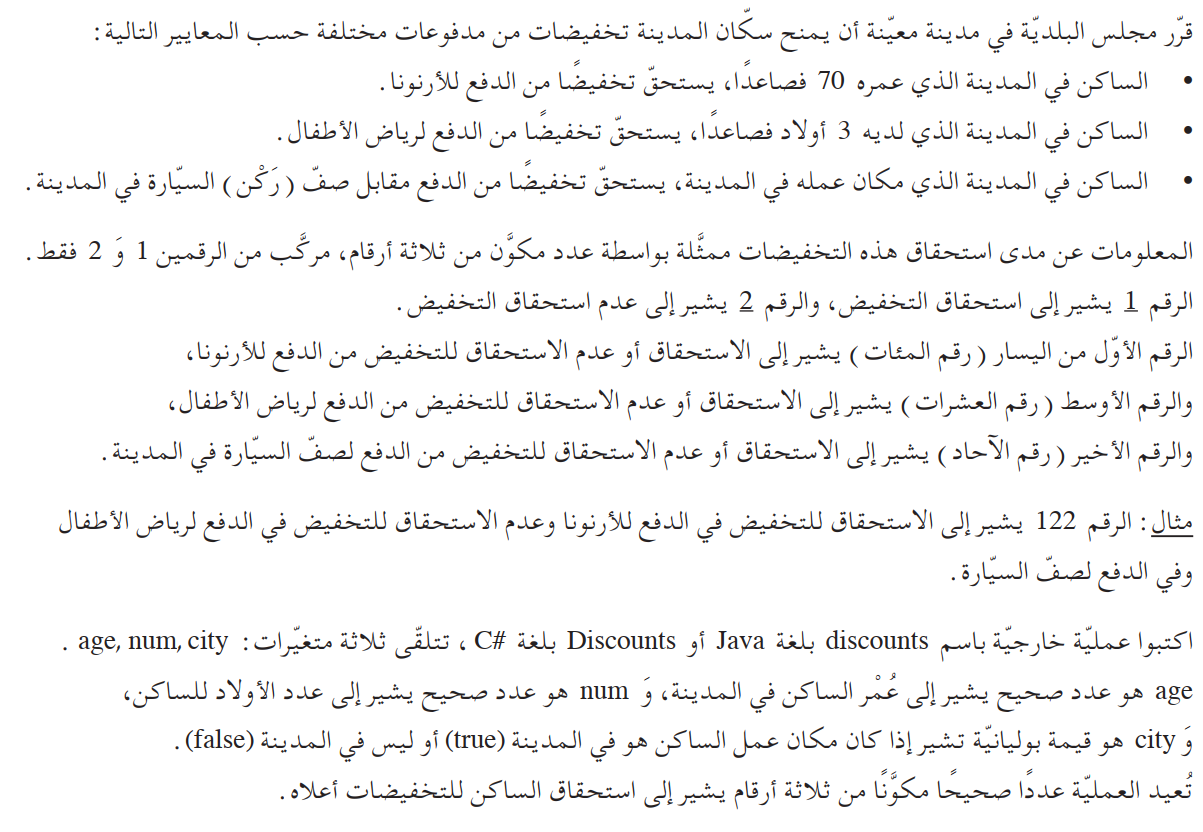
\includegraphics[width=1.1\textwidth]{../../../bagrut_questions/basics/functions_2023_899371_3.png}
\end{center}
\ifwithsols
\filbreak
\begin{boxSolution}[1]
\begin{english}
\begin{minted}{csharp}
public static int Discounts(int age, int num, bool city)
{
    int hundreds = 2, tens = 2, ones = 2;
    if (age >= 70)
    {
        hundreds = 1;
    }
    if (num >= 3)
    {
        tens = 1;
    }
    if (city)
    {
        ones = 1;
    }
    return hundreds * 100 + tens * 10 + ones;
}

public static void Main()
{
    int age = int.Parse(Console.ReadLine());
    int num = int.Parse(Console.ReadLine());
    bool city = bool.Parse(Console.ReadLine());
    Console.WriteLine(Discounts(age, num, city));
}
\end{minted}
\end{english}
\end{boxSolution}

\filbreak

\begin{boxSolution}[2]
\begin{english}
\begin{minted}{csharp}
public static int Discounts(int age, int num, bool city)
{
    int d = 0;
    if (age >= 70)
    {
        d += 100;
    }
    else
    {
        d += 200;
    }
    if (num >= 3)
    {
        d += 10;
    }
    else
    {
        d += 20;
    }
    if (city)
    {
        d += 1;
    }
    else
    {
        d += 2;
    }
    return d;
}
\end{minted}
\end{english}
\end{boxSolution}
\fi
\filbreak

\end{enumerate}

\vspace{1cm}
\begin{flushleft}
أرجو لكم وقتًا ممتعًا.

الأستاذ محمود اغبارية.
\end{flushleft}

\end{document}
